\documentclass{article}

%% This template is pieces of templates provided by Chi-Kit Lam for
%% CS395T in S2016, bits taken from
%% https://github.com/nykh/latex-shorthands/blob/master/myshorthands.tex, and %% other configs scrapped together over time. 
\PassOptionsToPackage{svgnames}{xcolor}
\usepackage[margin=2cm]{geometry}
\usepackage{float,graphicx,tabularx}
\usepackage[labelformat=simple]{subcaption}
\usepackage{eqparbox}
\usepackage{bbm}
\usepackage{leftidx}
\usepackage{mathtools}
\usepackage{semantic}
\usepackage[version=4]{mhchem} % chemical formulae
\usepackage{hyperref}
\usepackage{parskip}  %Extra space on new paragraph, no indent
\usepackage{graphicx}
\usepackage{natbib}
\usepackage{listings}
\usepackage{amsmath}
\usepackage{amssymb}
\usepackage{amsthm}

\renewcommand\thesubfigure{(\alph{subfigure})}

%%% Section Separators

\newcommand{\starhsep}{
\begin{center}
  $\ast$~$\ast$~$\ast$
\end{center}}

\newcommand{\clubhsep}{
\begin{center}
  $\clubsuit$~$\clubsuit$~$\clubsuit$
\end{center}}

%% Paired delimiters, use with \delim{*expression*}
\DeclarePairedDelimiter\abkt{\langle}{\rangle}
\DeclarePairedDelimiter\cbkt{\lbrace}{\rbrace}
\DeclarePairedDelimiter\rbkt{\lparen}{\rparen}
\DeclarePairedDelimiter\sbkt{\lbrack}{\rbrack}
\DeclarePairedDelimiter\abs{\lvert}{\rvert}
\DeclarePairedDelimiter\norm{\lVert}{\rVert}
\DeclarePairedDelimiter\floor{\lfloor}{\rfloor}
\DeclarePairedDelimiter\ceiling{\lceil}{\rceil}
\DeclarePairedDelimiterX\set[2]{\lbrack}{\rbrack}{#1 \colon #2}

%% Operators

\newcommand{\clapover}[2]{\overbrace{#1}_{\mathclap{#2}}}
\newcommand{\clapunder}[2]{\underbrace{#1}_{\mathclap{#2}}}

\DeclareMathOperator*{\argmin}{arg\,min}
\DeclareMathOperator*{\argmax}{arg\,max}
\DeclareMathOperator*{\minimize}{min}
\DeclareMathOperator{\supp}{supp}
\newcommand{\defeq}{\stackrel{\text{def}}=}

\DeclareMathOperator{\matrixtranspose}{T}
\newcommand{\T}{{\matrixtranspose}}
\DeclareMathOperator{\frobeniusnorm}{F}
\newcommand{\Fro}{{\frobeniusnorm}}
\DeclareMathOperator{\diag}{diag}

\DeclareMathOperator*{\E}{E}
\DeclareMathOperator*{\Var}{Var}
\DeclareMathOperator*{\Cov}{Cov}
\DeclareMathOperator*{\Corr}{Corr}
\DeclareMathOperator{\BinDist}{Bin}
\DeclareMathOperator{\GaussDist}{N}
\DeclareMathOperator{\PoisDist}{Pois}
\DeclareMathOperator{\UnifDist}{U}
\DeclareMathOperator{\erf}{erf} % error function.
\DeclareMathOperator{\sgn}{sgn}

\newcommand{\prox}{ \mathop{\mathrm{prox}} }
\newcommand{\enorm}[1]{\Vert #1 \Vert_2}

\DeclareMathOperator{\df}{d} % Differential form.
\DeclareMathOperator{\round}{\partial}

\DeclareMathOperator{\area}{area}
\DeclareMathOperator{\vol}{vol}

%% Variables. This may seem excessive but trust me it's quite nice

\newcommand{\eps}{\varepsilon}
\newcommand{\haat}{\widehat}

\newcommand{\bbA}{{\mathbb{A}}}
\newcommand{\bbB}{{\mathbb{B}}}
\newcommand{\bbC}{{\mathbb{C}}}
\newcommand{\bbD}{{\mathbb{D}}}
\newcommand{\bbE}{{\mathbb{E}}}
\newcommand{\bbF}{{\mathbb{F}}}
\newcommand{\bbG}{{\mathbb{G}}}
\newcommand{\bbH}{{\mathbb{H}}}
\newcommand{\bbI}{{\mathbb{I}}}
\newcommand{\bbJ}{{\mathbb{J}}}
\newcommand{\bbK}{{\mathbb{K}}}
\newcommand{\bbL}{{\mathbb{L}}}
\newcommand{\bbM}{{\mathbb{M}}}
\newcommand{\bbN}{{\mathbb{N}}}
\newcommand{\bbO}{{\mathbb{O}}}
\newcommand{\bbP}{{\mathbb{P}}}
\newcommand{\bbQ}{{\mathbb{Q}}}
\newcommand{\bbR}{{\mathbb{R}}}
\newcommand{\bbS}{{\mathbb{S}}}
\newcommand{\bbT}{{\mathbb{T}}}
\newcommand{\bbU}{{\mathbb{U}}}
\newcommand{\bbV}{{\mathbb{V}}}
\newcommand{\bbW}{{\mathbb{W}}}
\newcommand{\bbX}{{\mathbb{X}}}
\newcommand{\bbY}{{\mathbb{Y}}}
\newcommand{\bbZ}{{\mathbb{Z}}}
\newcommand{\bbone}{{\mathbbm{1}}}

\newcommand{\bfA}{{\mathbf{A}}}
\newcommand{\bfB}{{\mathbf{B}}}
\newcommand{\bfC}{{\mathbf{C}}}
\newcommand{\bfD}{{\mathbf{D}}}
\newcommand{\bfE}{{\mathbf{E}}}
\newcommand{\bfF}{{\mathbf{F}}}
\newcommand{\bfG}{{\mathbf{G}}}
\newcommand{\bfH}{{\mathbf{H}}}
\newcommand{\bfI}{{\mathbf{I}}}
\newcommand{\bfJ}{{\mathbf{J}}}
\newcommand{\bfK}{{\mathbf{K}}}
\newcommand{\bfL}{{\mathbf{L}}}
\newcommand{\bfM}{{\mathbf{M}}}
\newcommand{\bfN}{{\mathbf{N}}}
\newcommand{\bfO}{{\mathbf{O}}}
\newcommand{\bfP}{{\mathbf{P}}}
\newcommand{\bfQ}{{\mathbf{Q}}}
\newcommand{\bfR}{{\mathbf{R}}}
\newcommand{\bfS}{{\mathbf{S}}}
\newcommand{\bfT}{{\mathbf{T}}}
\newcommand{\bfU}{{\mathbf{U}}}
\newcommand{\bfV}{{\mathbf{V}}}
\newcommand{\bfW}{{\mathbf{W}}}
\newcommand{\bfX}{{\mathbf{X}}}
\newcommand{\bfY}{{\mathbf{Y}}}
\newcommand{\bfZ}{{\mathbf{Z}}}
\newcommand{\bfa}{{\mathbf{a}}}
\newcommand{\bfb}{{\mathbf{b}}}
\newcommand{\bfc}{{\mathbf{c}}}
\newcommand{\bfd}{{\mathbf{d}}}
\newcommand{\bfe}{{\mathbf{e}}}
\newcommand{\bff}{{\mathbf{f}}}
\newcommand{\bfg}{{\mathbf{g}}}
\newcommand{\bfh}{{\mathbf{h}}}
\newcommand{\bfi}{{\mathbf{i}}}
\newcommand{\bfj}{{\mathbf{j}}}
\newcommand{\bfk}{{\mathbf{k}}}
\newcommand{\bfl}{{\mathbf{l}}}
\newcommand{\bfm}{{\mathbf{m}}}
\newcommand{\bfn}{{\mathbf{n}}}
\newcommand{\bfo}{{\mathbf{o}}}
\newcommand{\bfp}{{\mathbf{p}}}
\newcommand{\bfq}{{\mathbf{q}}}
\newcommand{\bfr}{{\mathbf{r}}}
\newcommand{\bfs}{{\mathbf{s}}}
\newcommand{\bft}{{\mathbf{t}}}
\newcommand{\bfu}{{\mathbf{u}}}
\newcommand{\bfv}{{\mathbf{v}}}
\newcommand{\bfw}{{\mathbf{w}}}
\newcommand{\bfx}{{\mathbf{x}}}
\newcommand{\bfy}{{\mathbf{y}}}
\newcommand{\bfz}{{\mathbf{z}}}
\newcommand{\bfzero}{{\mathbf{0}}}
\newcommand{\bfone}{{\mathbf{1}}}
\newcommand{\bfGamma}{{\boldsymbol \Gamma}}
\newcommand{\bfDelta}{{\boldsymbol \Delta}}
\newcommand{\bfTheta}{{\boldsymbol \Theta}}
\newcommand{\bfLambda}{{\boldsymbol \Lambda}}
\newcommand{\bfXi}{{\boldsymbol \Xi}}
\newcommand{\bfPi}{{\boldsymbol \Pi}}
\newcommand{\bfSigma}{{\boldsymbol \Sigma}}
\newcommand{\bfUpsilon}{{\boldsymbol \Upsilon}}
\newcommand{\bfPhi}{{\boldsymbol \Phi}}
\newcommand{\bfPsi}{{\boldsymbol \Psi}}
\newcommand{\bfOmega}{{\boldsymbol \Omega}}
\newcommand{\bfalpha}{{\boldsymbol \alpha}}
\newcommand{\bfbeta}{{\boldsymbol \beta}}
\newcommand{\bfgamma}{{\boldsymbol \gamma}}
\newcommand{\bfdelta}{{\boldsymbol \delta}}
\newcommand{\bfeps}{{\boldsymbol \eps}}
\newcommand{\bfzeta}{{\boldsymbol \zeta}}
\newcommand{\bfeta}{{\boldsymbol \eta}}
\newcommand{\bftheta}{{\boldsymbol \theta}}
\newcommand{\bfiota}{{\boldsymbol \iota}}
\newcommand{\bfkappa}{{\boldsymbol \kappa}}
\newcommand{\bflambda}{{\boldsymbol \lambda}}
\newcommand{\bfmu}{{\boldsymbol \mu}}
\newcommand{\bfnu}{{\boldsymbol \nu}}
\newcommand{\bfxi}{{\boldsymbol \xi}}
\newcommand{\bfpi}{{\boldsymbol \pi}}
\newcommand{\bfrho}{{\boldsymbol \rho}}
\newcommand{\bfsigma}{{\boldsymbol \sigma}}
\newcommand{\bftau}{{\boldsymbol \tau}}
\newcommand{\bfupsilon}{{\boldsymbol \upsilon}}
\newcommand{\bfphi}{{\boldsymbol \phi}}
\newcommand{\bfchi}{{\boldsymbol \chi}}
\newcommand{\bfpsi}{{\boldsymbol \psi}}
\newcommand{\bfomega}{{\boldsymbol \omega}}

\newcommand{\calA}{{\mathcal{A}}}
\newcommand{\calB}{{\mathcal{B}}}
\newcommand{\calC}{{\mathcal{C}}}
\newcommand{\calD}{{\mathcal{D}}}
\newcommand{\calE}{{\mathcal{E}}}
\newcommand{\calF}{{\mathcal{F}}}
\newcommand{\calG}{{\mathcal{G}}}
\newcommand{\calH}{{\mathcal{H}}}
\newcommand{\calI}{{\mathcal{I}}}
\newcommand{\calJ}{{\mathcal{J}}}
\newcommand{\calK}{{\mathcal{K}}}
\newcommand{\calL}{{\mathcal{L}}}
\newcommand{\calM}{{\mathcal{M}}}
\newcommand{\calN}{{\mathcal{N}}}
\newcommand{\calO}{{\mathcal{O}}}
\newcommand{\calP}{{\mathcal{P}}}
\newcommand{\calQ}{{\mathcal{Q}}}
\newcommand{\calR}{{\mathcal{R}}}
\newcommand{\calS}{{\mathcal{S}}}
\newcommand{\calT}{{\mathcal{T}}}
\newcommand{\calU}{{\mathcal{U}}}
\newcommand{\calV}{{\mathcal{V}}}
\newcommand{\calW}{{\mathcal{W}}}
\newcommand{\calX}{{\mathcal{X}}}
\newcommand{\calY}{{\mathcal{Y}}}
\newcommand{\calZ}{{\mathcal{Z}}}

%% Special Group Aliases

\DeclareMathOperator{\groupGF}{GF}
\DeclareMathOperator{\groupGL}{GL}
\DeclareMathOperator{\groupSL}{SL}
\DeclareMathOperator{\groupO}{O}
\DeclareMathOperator{\groupSO}{SO}
\DeclareMathOperator{\groupU}{U}
\DeclareMathOperator{\groupSU}{SU}
\DeclareMathOperator{\groupE}{E}
\DeclareMathOperator{\groupSE}{SE}

\mathlig{---}{\text{---}}

%% Some sane listings defaults

\usepackage{color}

\definecolor{mygreen}{rgb}{0,0.6,0}
\definecolor{mygray}{rgb}{0.5,0.5,0.5}
\definecolor{mymauve}{rgb}{0.58,0,0.82}

\lstset{ %
  backgroundcolor=\color{white},   % choose the background color; you must add \usepackage{color} or \usepackage{xcolor}
  basicstyle=\footnotesize,        % the size of the fonts that are used for the code
  breakatwhitespace=false,         % sets if automatic breaks should only happen at whitespace
  breaklines=true,                 % sets automatic line breaking
  captionpos=b,                    % sets the caption-position to bottom
  commentstyle=\color{mygreen},    % comment style
  deletekeywords={...},            % if you want to delete keywords from the given language
  escapeinside={\%*}{*)},          % if you want to add LaTeX within your code
  extendedchars=true,              % lets you use non-ASCII characters; for 8-bits encodings only, does not work with UTF-8
  frame=single,                    % adds a frame around the code
  keepspaces=true,                 % keeps spaces in text, useful for keeping indentation of code (possibly needs columns=flexible)
  keywordstyle=\color{blue},       % keyword style
  language=Octave,                 % the language of the code
  otherkeywords={*,...},           % if you want to add more keywords to the set
  numbers=left,                    % where to put the line-numbers; possible values are (none, left, right)
  numbersep=5pt,                   % how far the line-numbers are from the code
  numberstyle=\tiny\color{mygray}, % the style that is used for the line-numbers
  rulecolor=\color{black},         % if not set, the frame-color may be changed on line-breaks within not-black text (e.g. comments (green here))
  showspaces=false,                % show spaces everywhere adding particular underscores; it overrides 'showstringspaces'
  showstringspaces=false,          % underline spaces within strings only
  showtabs=false,                  % show tabs within strings adding particular underscores
  stepnumber=2,                    % the step between two line-numbers. If it's 1, each line will be numbered
  stringstyle=\color{mymauve},     % string literal style
  tabsize=2,                     % sets default tabsize to 2 spaces
  title=\lstname                   % show the filename of files included with \lstinputlisting; also try caption instead of title
}


%%% style.sty ends%%%

\title{SDS 385 Exercise Set}
\author{Kevin Song}
\date{\today}

\begin{document}

\maketitle

The Laplacian matrix has the following form (where $d(i)$ is the degree of
vertex $i$):

\begin{equation}
  \calL_{i,j} =
  \begin{cases}
    d(i)  & \text{ for } i = j\\
    -1    & \text{ for } i \text{ adjacent to } j\\
    0     & \text{otherwise}
  \end{cases}
  \label{eq:Lelem}
\end{equation} 

If we let $D_i$ denote the $i$th column of $D$, then the $i,j$th element of
$D^TD$ is equal to $D_i \cdot D_j$. We now seek to show that $D_i \cdot D_j$ is
equivalent to the $i,j$th element of $\calL$ as described in Equation
\eqref{eq:Lelem}.

\begin{proof}
  From the description in the text, $D_i$ has nnz (number of nonzero elements)
  equal to the degree of vertex $i$. Let $nzi(D_i)$ be the nonzero indicies of
  $D_i$, that is, if $j \in nzi(D_i)$, then $D_{ij}$ (the $j$-th element of
  $D_i$) is equal to either plus or minus one. Then

  \begin{align*}
    D_i \cdot D_i = \sum_{j \in nzi(D_i)} D_{ij}^2 = \sum_{j \in nzi(D_i)} 1 = \text{nnz}(D_i) = d(i)
  \end{align*}

  So $D^TD_{i,j} = d(i)$ when $i = j$, which matches Equation~\eqref{eq:Lelem}.

  Now suppose $i \neq j$. If vertex $i$ and vertex $j$ do not share any edges,
  then there does not exist a $k$ such that $D_{ik} \neq 0$ and $D_{jk} \neq 0$.
  Then $D_i \cdot D_j$ is necessarily zero, in agreement with
  Equation~\eqref{eq:Lelem}

  Now suppose that the vertices share one (and exactly one) edge. Suppose this
  edge is edge $k$. Then if $i < j$, $D_{ik} = 1$ and $D_{ji} = -1$, or vice
  versa if $i > k$. In either case, $D_i^TD_j = -1$.
\end{proof}

Since they are elementwise equal, $\calL = D^TD$, and so $x^T\calL x = x^TD^TDx
= \norm{Dx}_2^2$.

This minimization problem can now be expressed as

\[
  \minimize\limits_{x \in \mathbb{R}^n} \frac{1}{2} (y - x)^T(y - x) + \frac{\lambda}{2} (Dx)^T(Dx)
\]

After some algebraic manipulation, we find that this is equivalent to
\[
  \minimize\limits_{x \in \mathbb{R}^n} \frac{1}{2}  x^T(\lambda D^TD + I^TI) x
  - y^Tx + \frac{y^Ty}{2}
\]

Since this is a quadratic form, the minimum is found by solving

\begin{equation}
  (\lambda D^TD + I) \hat{x} = y
  \label{eq:optprob}
\end{equation}


so we choose $b = y$ and $C = (\lambda D^TD + I)$

\section*{Comparisons!}

I chose to solve this with a direct solver, Gauss-Seidel, and Jacobi Iteration.
Running \texttt{solvers.py} in the code directory will run all three solvers,
and generate plot comparisons with the original.

In terms of running speed, Gauss-Seidel was hideously slow. Direct solves with
SuperLU were decently fast, at just under a second apiece, and Jacobi iteration
blew everything else away at about 0.1s per solve. I attribute the issues with
Gauss-Seidel to the lack of a good sparse triangular solver in SciPy: without
a solver that can take advantage of a triangular matrix to do forward solves,
the fastest way to create a solution is to invert the lower triangular matrix,
which takes eons because it is does not account for the triangular structure and
instead does an LU factorization. The running speeds are summarized in Table
\ref{tab:runtime}.

\begin{table}[h]
  \centering
  \begin{tabular}{|c|c|}
    \hline
   Direct Solve & 0.777 seconds\\ \hline
   Gauss-Seidel & 43.99 seconds\\ \hline
   Jacobi Iteration & 0.08 seconds\\ \hline
  \end{tabular}
  \caption{Time to solve a single system, averaged over 3 runs}
  \label{tab:runtime}
\end{table}

The solutions show a residual of about $10^{-14}$ from the problem defined in
Equation~\eqref{eq:optprob}, and no greater difference than $10^{-15}$ from each
other elementwise (i.e. the inf norm of the difference of any two solutions is
less than $10^{-15}$), which suggests that the solutions are mostly identical. A
plot of the solutions, shown in Figure~\ref{fig:f1}, shows that they are
qualitatively the same. The plot in Figure~\ref{fig:f2}, of the differences
between the smoothed and actual, shows that none of the techniques have exactly
the same answer.

\begin{figure}[h]
  \centering
  \begin{subfigure}{0.45 \textwidth}
    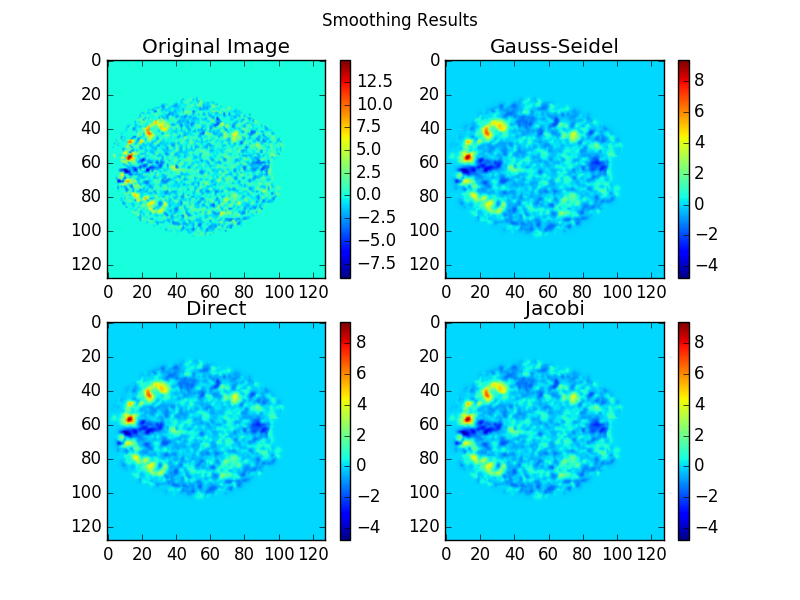
\includegraphics[width=\textwidth]{figure_1.png}
    \caption{A plot of the spatially-smoothed results.\\ Qualitatively, all
      methods arrive at the same result.}
    \label{fig:f1}
  \end{subfigure} 
  \begin{subfigure}{0.45 \textwidth}
    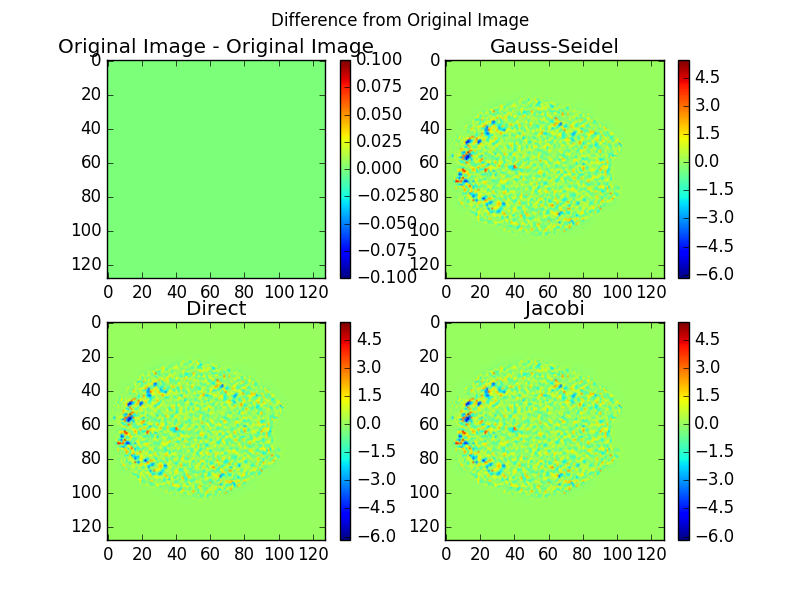
\includegraphics[width=\textwidth]{figure_2.png}
    \caption{Differences of the spatially-smoothed data from the actual data.
      Minor differences are present, but they are on the order of $10^{-15}$.
      Crucially, each method gets a different result.}
    \label{fig:f2}
  \end{subfigure} 
\end{figure}

\section{Graph fused lasso}

Since I spent entirely too much time on the above section, I chose to implement
the slow ADMM.

\begin{figure}[h]
  \centering
  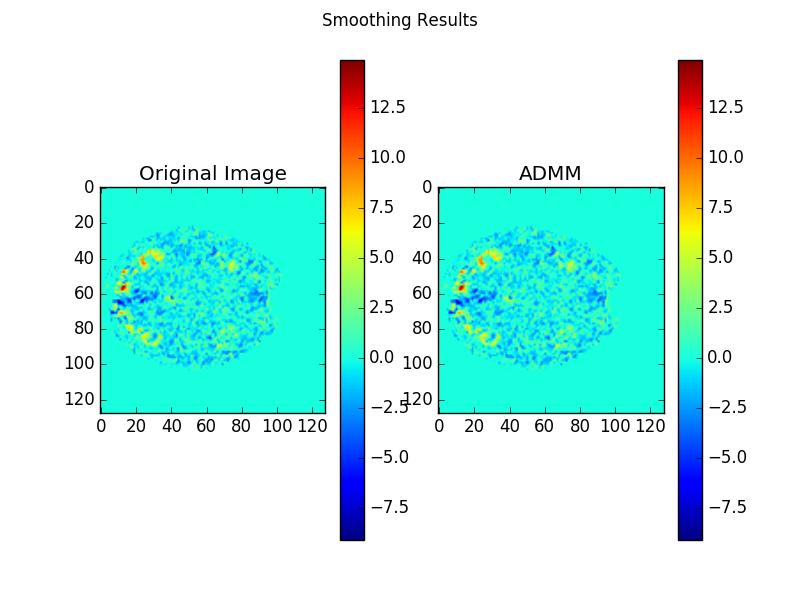
\includegraphics[width=0.8\textwidth]{figure_3}
  \caption{ADMM versus original data}
  \label{fig:f3}
\end{figure}

\end{document}
